\documentclass[jou,apacite]{apa6}

\title{psiTurk: A framework for running behavioral experiments online}
\shorttitle{APA style}

\twoauthors{Author One}{Author Two}
\twoaffiliations{Institute of Psychology}{Freud's Institute}

\abstract{psiTurk is really great and you should use it.}

\rightheader{APA style}
\leftheader{Author One}

\begin{document}
\maketitle
\section{Introduction (AC)}

Online experiments are growing in popularity. 
They offer a number of advantages over lab-based experiments, as well as novel technical and experimental challenges.

psiTurk is a framework of software and web services that facilitate the creation, running, and dissemination of web-based experiments.
It presently relies on Amazon Mechanical Turk to recruit and pay participants on the web.
It solves a number of technical requirements including serving an experiment on the web, saving experimental data, and restricting the participant pool according to the experimenter's needs.
The principal goal of this framework is thus to handle common technical challenges so that researchers can focus on the development and dissemination of online experiments.

\section{Web-based behavioral research}

\subsection{Survey of researchers' needs (AR)}

In month, 2014 we conducted a survey to assess the methods and needs of behavioral researchers with respect to online experiments.
We got some great feedback from the community, with 201 people responding.
We heard from a wide range of academic fields.
While most respondents (unsurprisingly) hailed from psychology, we also heard from researchers in linguistics, marketing, neuroscience, and economics.

Most researchers (85\%) had some experience collecting behavioral data online in their labs.
 First, there is a clear interest in and acceptance of the use of online data in research.
This is interesting because even a few years ago there was much more skepticism that random people doing your experiment over the Internet would give valid data.
Nearly 40\% suggested they treat papers reporting data collected online identically to that collected in a lab.
Nearly all respondents selected large sample sizes (93\%) and a more diverse population (98\%) as potential advantages of collecting data online, with most listing a more diverse population (60\%) and cost (75\%) as factors as well.
However, some researchers felt that online data is unreliable (35\%), the population is unrepresentative (25\%), and the technology required to collect data online is too complex (26\%).

Half of respondents also stated that the experiment designs they were interested in do not work well online, and researchers outside the US indicated having difficulties using services like Amazon Mechanical Turk.
Second, it appears there remain significant software challenges in helping most researchers do behavioral data collection online.
The majority of our respondents listed Qualtrics, a service for conducting online surveys, as the tool they were currently most likely to use.
At the same time, 79\% of respondents were interested in running full experiments online including multiple trials, fixation crosses, etc.

\begin{figure*}[tp]
\centering
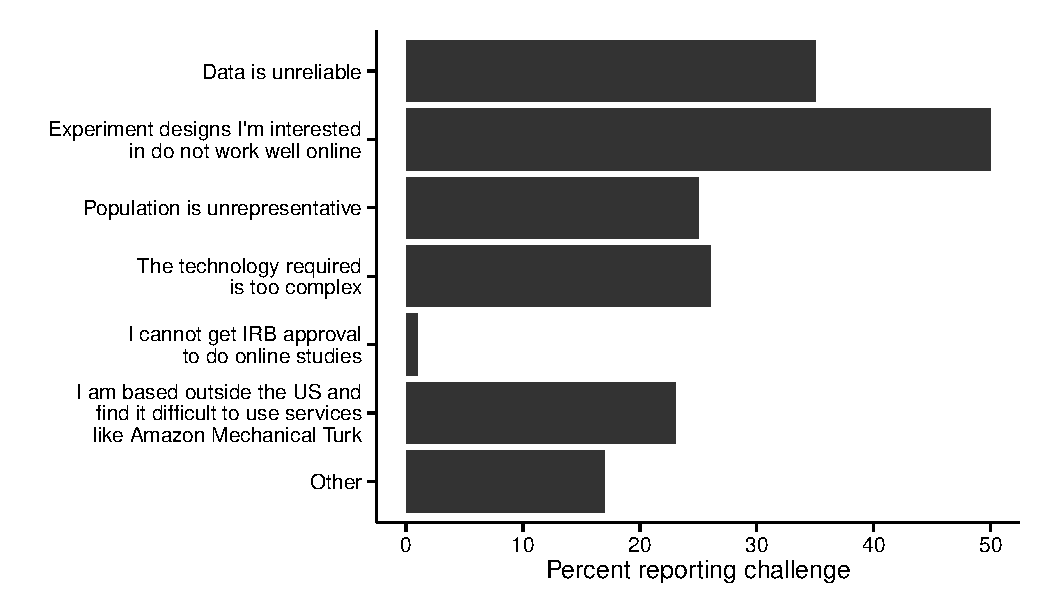
\includegraphics[scale=.75]{challenges.pdf}
\label{fig:challenges}
\caption{Challenges faced by 201 researchers who completed our survey on collecting behavioral data online.}
\end{figure*}

The vast majority (94\%) of those surveyed indicated they were interested in new tools which simplified online data collection.
Of the features people hoped such software would include, 90\% listed the ability to block repeat participation, and 70\% listed the ability to automatically pay people (incidentally, these are all features of our lab's psiTurkpackage).
In addition, 64\% said the availability of example code that one could use to jump-start their own experiment design was important (also a feature of psiTurk's Experiment Exchange).
A majority of participants thought a cloud-based solution with a GUI interface would be the preferred form for this type of software to take and 64\% indicated a general lack of experience or knowledge about web-based programming (e.g., Javascript, HTML, etc).
Interestingly, this is currently not how psiTurk works! (Stay tuned though, as we are currently developing greater cloud-compatibility.)

Anyway, the take home seems to be that the acceptance of online data collection is increasing, but the tools for doing this are still lacking in ways most relevant to behavioral researchers.
We conducted this study exactly because our lab is working on open-source tools to help with this.
While our approach doesn't solve every problem that exists in the community, it does seem to tap many of the concerns these respondents have.
This is definitely an interesting space for future development and there seems to be a market for tools which simplify online data collection and which provide services for those outside the US who can't leverage the Amazon Mechanical Turk platform.


\subsection{Amazon Mechanical Turk (AMT)} 

Amazon Mechanical Turk (AMT) is an online platform that lets you post a wide variety of tasks to a large pool of participants.
Instead of spending weeks to run experiments in the lab, it lets you collect data of a large number of people within a couple of hours.
Workers get paid a fixed amount for each HIT which is determined by the requester.

\subsubsection{From the worker's perspective (JVM)}
AMT functions as an online listing service for online jobs.
Workers search through a list of tasks, known as Human Intelligence Tasks (HITs). 
When a worker examines a particular task, they are able to see metadata about the task, such as its title and how much it pays, and a website provided by the requester inside a web frame.
This website serves as an advertisement for the task and must be hosted either by Amazon or on the requester's hosted servers.
Once a worker has accepted a HIT, he or she agrees to complete it within a particular amount of time.
The actual task is again served either from Amazon or the requester's own hosted service.
The hosting both serves the job to the worker and collects data.
Finally, the worker is returned the AMT worker page to be credited and continue to another HIT.

\subsubsection{From the requester's perspective (TMG)}
Requesters can also make bonus payments to specific workers. Amazon collects a 10\% fee for each payment.
AMT provides some very basic templates that you can use to design HITs (particularly questionnaires), but these will most likely not serve your purposes as an experimenter.
The psiTurk toolbox is designed to help you run fully-customized and dynamic web-experiments on AMT.
Specifically, it allows you to:
1. Run a web server for your experiment
2. Test your experiment
3. Interact with AMT to recruit, post HITs, filter, and pay participants (AMT workers)
4. Manage databases and export data
psiTurk also includes a powerful interactive command interface that lets you manage most of your AMT activity.


\subsection{What problems does psiTurk solve? (AC)}

Brief overview of how psiTurk addresses needs/challenges raised in the previous sections, before going on to a more detailed walkthrough in the next section.

Flexible database options

Server-side solutions

Automatic bonusing

No need to install, configure and maintain complex webserver software (e.g., Apache, MySQL)

Minimize security issues since server only runs while you want to collect data

No need for dedicated server

Ability to filter browsers, iPhones, tablets, etc. 

Custom routes

Nicer interface to Mturk than Mturk 

Automatically fill in conditions randomly and evenly

Templates (consent, instructions, errors, debrief)

Includes industry standards (Bootstrap, jQuery, d3, etc) 

Prevent same worker from performing your experiment multiple times

Simplifies paying participants quickly, including bonuses

The psiTurk Ad Server is a cloud-based solution for delivering ads to participants securely, while providing experiments useful information about who is taking their experiment, where they are connecting from, and possibly what other experiments they have completed.


%\begin{table*}[t]
%\caption{default}
%\begin{center}
%\begin{tabular}{|l|l|l|}
%Category & Issue & psiTurk solution \\
%\hline
%Participant pool & Preventing repeated participation in same experiment & Database \\
%\end{tabular}
%\end{center}
%\label{default}
%\end{table*}%



\section{Overview of the psiTurk system}


\subsection{Command line interface: Managing HITs and serving the experiment (AR)}

PsiTurk runs as a command line interface (CLI) within a standard terminal window.
There are several advantages to designing psiTurk as a simple CLI beyond its efficiency of use. This
design makes the user-interface code clear and easy to read and write, allowing newcomers to quickly
understand and contribute to the open-source project. Integrating a new feature into the interface
is as simple as describing the syntax and functioning of a new command. The CLI also ensures that
psiTurk is easy to interact with not just on a laptop or desktop but also on a remote server or in
the cloud, where users may have terminal-only access.
 
Entering
\texttt{psiturk} at the command line in any directory containing a psiTurk project launches the
psiTurk CLI.
The psiTurk CLI features a colorized prompt that provides important information at a glance, such as
whether the server is running and the number of HITs currently running on MTurk. 

\subsubsection{Managing HITs}
Commands are
organized into groups based on their function, following a general ``\texttt{command subcommand
arguments}'' format. For example, one can create a HIT by typing \texttt{hit create <\# assignments>
<payment amount> <duration>} or list all active HITs with \texttt{hit list -{}-active}, and can
restart the server with \texttt{server restart} or open the server log with \texttt{server log}. Tab
completion makes it quick to type commands, and the \texttt{help} command can be used to show
details on the usage of any command. The straighforward and consistent syntax of the CLI allows
users to perform a wide variety of tasks--from creating HITs and paying workers, to launching Amazon
Web Services database instances, to opening an experiment in a browser for debugging--that
would otherwise be spread across a number of websites and programs. In most cases, a user of the
psiTurk CLI will never have to log into the MTurk website except to add money to their MTurk
requester account.
Easily switch between AMT's sandbox and live site.


\subsubsection{Serving an experiment}
psiTurk experiments can be hosted on almost anything that has an internet connection and a public port, such as an office computer or laptop.
You'll need a static IP to prevent your experiment's URL from changing. 
Users without one (e.g., most home users) can use a dynamic DNS service to forward a URL to their dynamic IP.
Here's a list of free DDNS providers.
You also may need to forward a port from your home routers to you personal computer.
To run your experiment in a web browser you need to have at least some basic web programming skills (especially using HTML, CSS, and JavaScript).
Once you mastered the basics, you can take advantage of the vast number of libraries and tools that can help you to build sharp and sophisticated experiments with the support of a large community of users.
To get you started, psiTurk provides a fully functioning example experiment (Getting up and running with the basic Stroop task) that you can use as a template for your own study.


\subsection{The Ad server}

PsiTurk helps an experimenter in both hosting the ad and delivering the experiment.
First, PsiTurk provides a cloud service at \texttt{psiturk.org} for serving ads to workers.
This service serves the ads with appropriate SSL certificates, something which can be difficult on many server configurations.\footnote{SSL certification has recently become a requirement for hosting content within an \texttt{iframe} on \texttt{mturk.com}.}
Second, the PsiTurk web framework allows you to easily build and host your own experiment, running on your server or laptop and saving workers' data either to your own database  or to \texttt{psiturk.org}.
This gives experimenters complete flexbility in terms of content while also offering a suite of tools to make experiment development easy.

SSL hosted Ad Server removes need to deal with complex web security issues (https, data mining on workers) 
Participants recruited via Mechanical Turk first interact with your task via ads. Ads are simply the digital version of hanging a poster or flyer around your university building in order to recruit participants. Technically, ads are snippets of HTML code that describe what your task is about and what you're offering for compensation. As a result, they are the front line for any subject recruitment online. It's easy to overlook the importance of a good ad, and making that ad visible to as many participants as possible.




%Extendable Python based API: easily add new functionality
%
%Library of experiments you can adapt or replicate
%
%Fully open-source development helps catch bugs
%
%Since everything runs locally easy to debug/test (even w/o Internet!)
%
%Run experiments on local computer (via tunnel) (can run offline and online)
%
%Perfect for laboratory-based courses with undergrads (replicating studies)



\subsection{Javascript library \emph{psiTurk.js} (DBM)}

The javascript library \emph{psiTurk.js} enables interaction with the server from the client-side (javascript) experiment code.
The goal of the library is to handle the most common functionality of psiTurk-based web experiments, without imposing any additional requirements on the structure or design of the experiments themselves.
Researchers can draw on a vast array of javascript libraries to design their experiment, while using psiTurk.js to save data and notify the server of changes in a participant's status.

Figure X shows javascript code from an experiment script (\emph{task.js}). 
\emph{psiTurk.js} currently performs the following functions:

\begin{enumerate}

\item \textbf{Tracking a participant's progress in an experiment.} psiTurk records changes in a participant's status as they move through an experiment. 
Some of these status changes are automatic, e.g., when a participant is assigned to a condition or if they quit an experiment early. 
Two additional status changes are initiated by the client-side experiment code using psiTurk.js functions.
First, since experiments typically begin with an instructional phase, calling the function \texttt{psiturk.finishInstructions()} upon completion of this phase will save the participant's status as having begun the main experiment.
If the participant attempts to quit the experiment after that point, they will receive a warning that they will not be able to restart the experiment and may forgo payment.
Second, successful completion of the experiment is signaled by calling \texttt{psiturk.completeHIT()}, which closes the experiment and redirects the participant to the AMT page to submit their HIT.

\item \textbf{Saving experimental data.} Experiment code can save data in two formats.
\texttt{psiturk.recordTrialData} takes any array of values as input and appends it to a list of ``trial" data.
This data structure is meant for sequential data that may be collected over the course of multiple trials or blocks, where each line corresponds to a new measurement.
However, the format of this data is defined by the experimenter and is saved in the database as a single JSON object.

In contrast, \texttt{psiturk.recordUnstructuredData} is used to record (key, value) pairs, where the key is uniquely defined within the experiment.
This format is useful for survey questions or other one-time measurements, e.g., (\emph{Age}: 24).

Importantly, both functions above simply record the data in the appropriate format on the client-side.
When the experimenter wishes to save the data to the server they call \texttt{psiturk.saveData}.

\item \textbf{Automatic recording of browser interaction.} 
One general shortcoming of web experiments is greater uncertainty about a participant's testing environment and engagement with the experiment.
Unlike lab computers where undesired behaviors can be prevented, a person is always able to close a web browser, switch to different applications, or change other aspects of their experience.
However, standard methods exist for recording many aspects of a user's interaction with a web browser, and this data can be useful for 1) tracking how an experiment was actually displayed, and 2) the level of a participant's engagement.

For example, although it is possible to set the initial size of a browser window, a web participant can change the dimensions of the window, potentially obscuring or altering how the experiment is displayed.
\emph{psiTurk.js} automatically records these changes in the size of the window.
Similarly, the experiment can choose to switch focus away from the experiment window (e.g., to another browser window or a different application).
\emph{psiTurk.js} automatically records every time that the experiment window loses and gains the participant's focus.
This ``event data" is automatically recorded and saved to the database whenever \texttt{psiturk.saveData} is invoked.

\end{enumerate}

\emph{psiTurk.js} can also preload html pages and images.
Finally, it has a basic structure for presenting instructional pages.

\subsection{Experiment exchange}

psiTurk's experiment exchange is like an "app store" for experiment designs. 

Experiment exchange, "Get a head start", "friction-free replication", 

Standardization across labs/research groups aids replicability/code sharing


Share your code, help others replicate, or check out someone else's experiment as a starting place for coding your own. The experiment exchange also allows researchers to quickly download psiTurk-compatible experiments and re-run them online. Same population, same task code, direct replication, better science.
The experiment exchange allows researchers to share the code for psiTurk-compatible experiments. Other researchers can easily download the code from the exchange and re-run them online using the same population and task code. In addition, researchers can use the experiment exchange to learn about the code used in other people's experiments. 


\section{What are the limitations of psiTurk? (TMG)}

Restriction to AMT

No Windows

doesn't force particular javascript gui stuff

multiperson real-time experiments (Doug?) 

Showing videos is difficult (flash? html5? Slow connections? reload videos?)

How to pay people when they don't finish hit completely?


\section{Future directions}

counterbalancing (integrate PlanOut (Facebook's counterbalancing tool)) (DH)

Optimal Experimental Design/ Design of Experiments tools

Better multi-person/multi-session exp (websockets; doug?)?
Automate catch trials? How far did the worker get? Do we count them in the N? 
Limiting/throttling number of people doing the experiment at once
Video support

\bibliography{sample}

\end{document}
